\documentclass[12pt, letterpaper]{article}
\usepackage[utf8]{inputenc}
\usepackage[pdftex]{graphicx}
\usepackage{xspace}
\graphicspath{ {/home/tobiasjenegger/Documents/summary/} }
\title{Radius/Momentum Calculation for S444 Experiment February 2020 - Overview}
\author{Tobias Jenegger}

\begin{document}
\begin{titlepage}
\maketitle
\end{titlepage}
\subsection{The Setup}
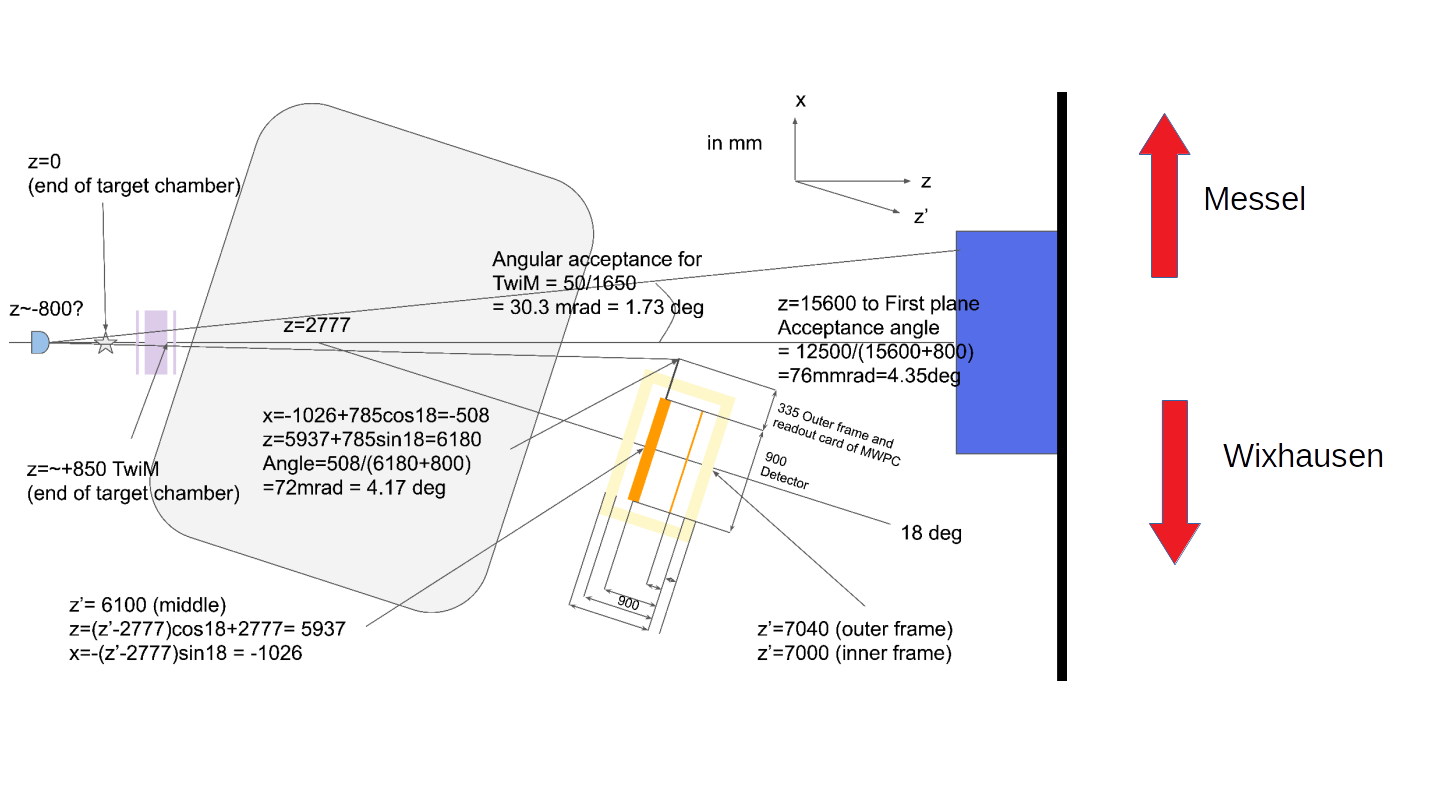
\includegraphics[width=1.2\textwidth]{mes_wixh.png}
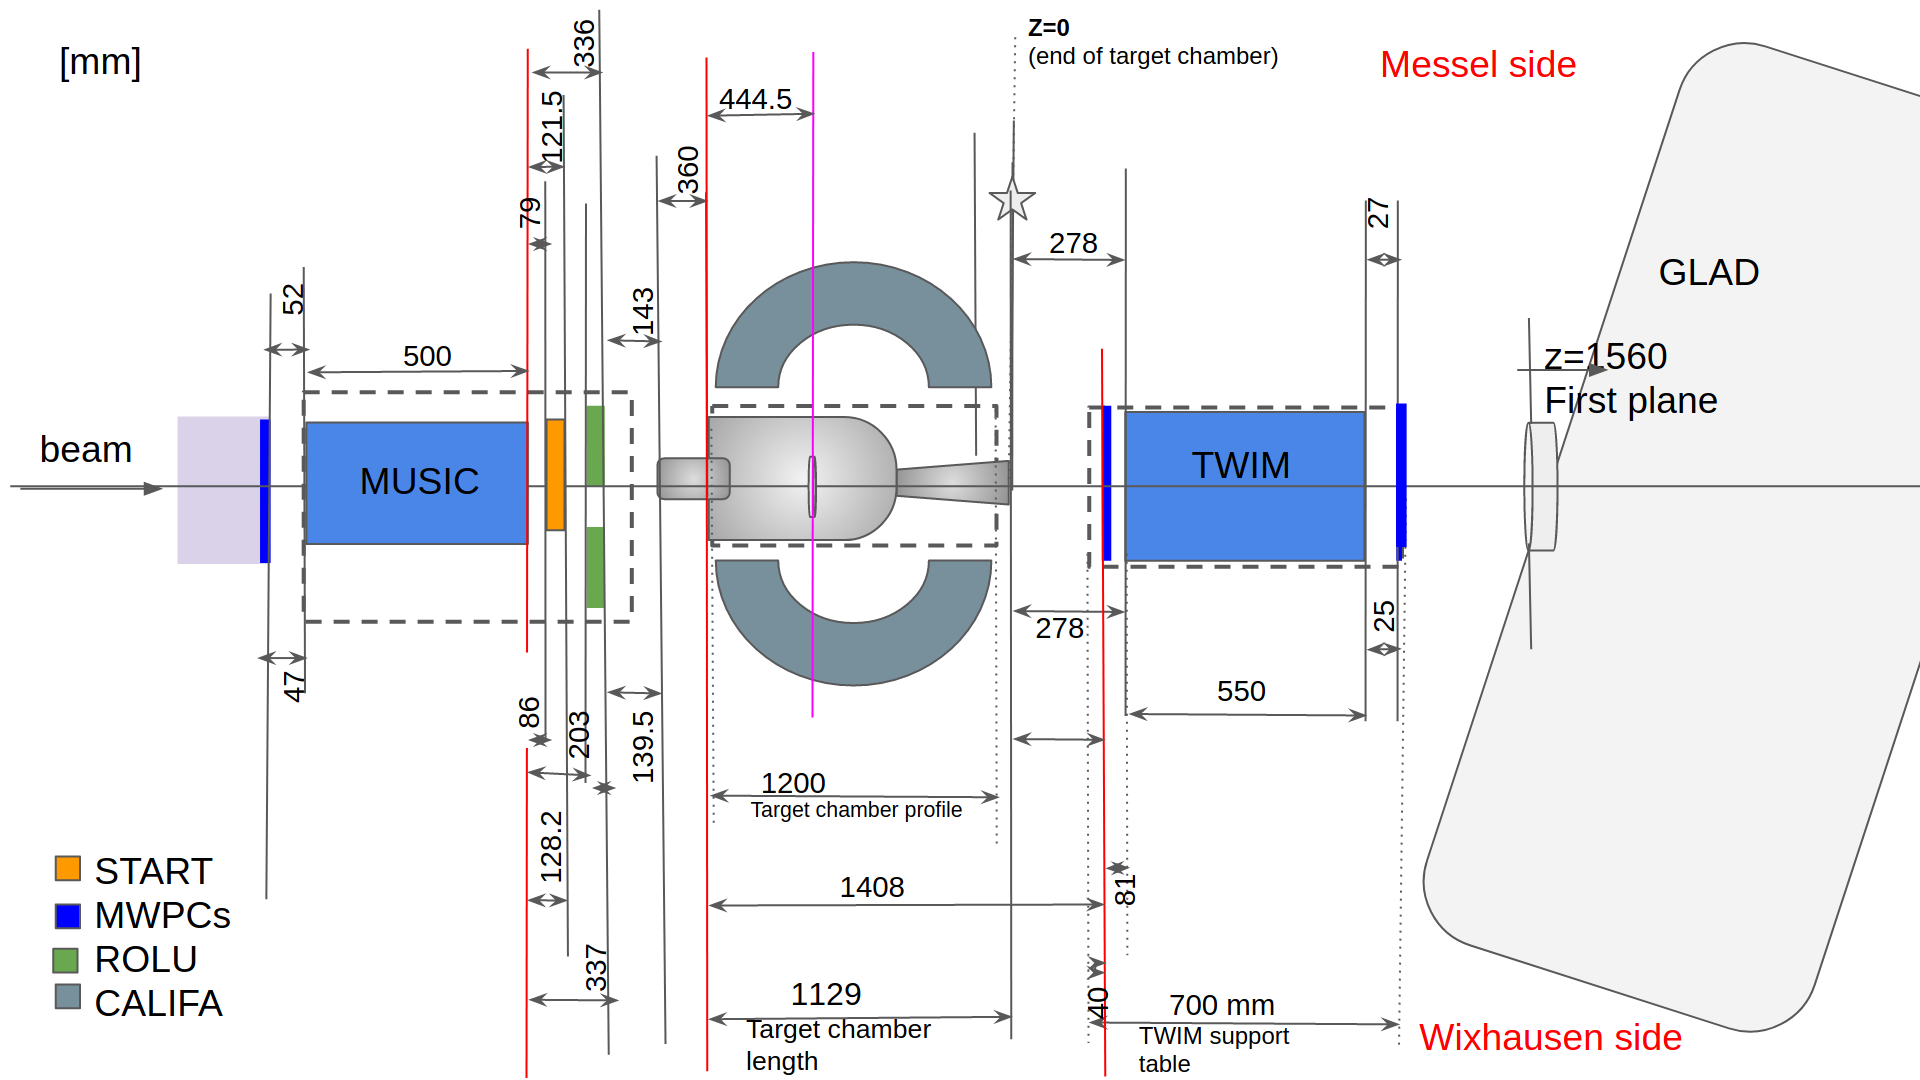
\includegraphics[width=1.2\textwidth]{SETUP_around_Target.png}
\section{Geometry and relative position of the detectors in the beam direction}
Here, the positions are given for the s444 and s467 experiments\\
\\
z position of the MWPC0: \hspace{10mm} zMW0 = -2520 mm\\
z position of the target: \hspace{10mm} zT = -684.5 mm\\
z position of the MWPC1 in front of the Twin-MUSIC:  \hspace{10mm}   zM1 = 279 mm \\
z position of the middle of the Twin-MUSIC:  \hspace{10mm}  zTwin = 553 mm\\
z position of the MWPC2 after the Twin-MUSIC:  \hspace{10mm}   zM2 = 854 mm\\
$\alpha$ tilted angle of GLAD (14 degrees):   \hspace{10mm} = 0.244 rad\\
effective length of GLAD:  \hspace{10mm}   L\textunderscore eff = 2067 mm\\
z middle of GLAD  \hspace{10mm}  zGm = 2577mm\\
horizontal of the central path (18 degree) \hspace{10mm}   $\theta$\textunderscore out0 = pi/10 rad\\
z position of the MWPC3 after GLAD   \hspace{10mm}  zM3 = 5937 mm\\
z position of the ToFwall          \hspace{10mm}     zToFW = 6660.2 mm\\
\\
Correspondence between the GLAD current and the magnetic field:  I = 3584 A, B = 2.2 T \\
\\
Positions of the TOFWPads:\\
1 $\Rightarrow$ Messel\\
27$\Rightarrow$ Wixhausen \\

\section{RUNS used for calibration = SWEEP RUNS without target}

\begin{center}
	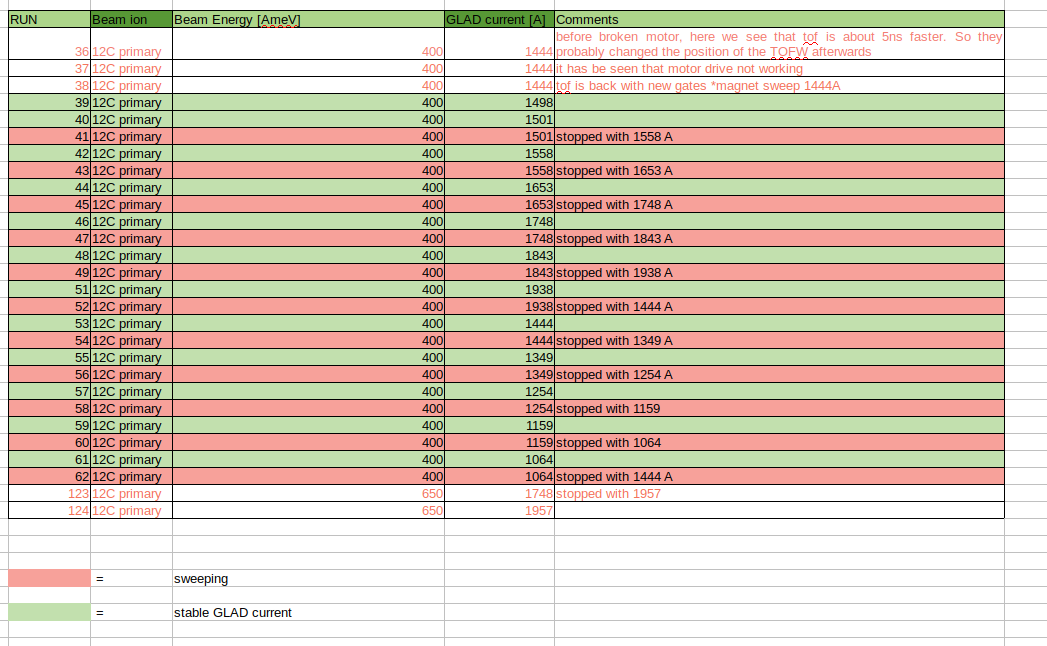
\includegraphics[width=1.2\textwidth]{runs_screenshot.png}
\end{center}

\subsubsection{Other RUNS used for various checks:}
RUN 70: 2 cm C target\\
RUN 80: 10.86 mm C target\\
RUN 81: 24.53 mm CH2 target\\
RUN 67: 24 mm CH2 target \\
RUN 68: 1 cm C target \\
RUN 79: 12.29 mm CH2 target\\
RUN 75: 21.98mm C target\\
\\

\section{Methods for flightpath reconstruction in the (x,z) plane}
\subsection{The "Kickplane" method}
\subsubsection{From MW0 to the entrance of GLAD, the ion is following a straight line}\label{sssec:num1}
\begin{center}
	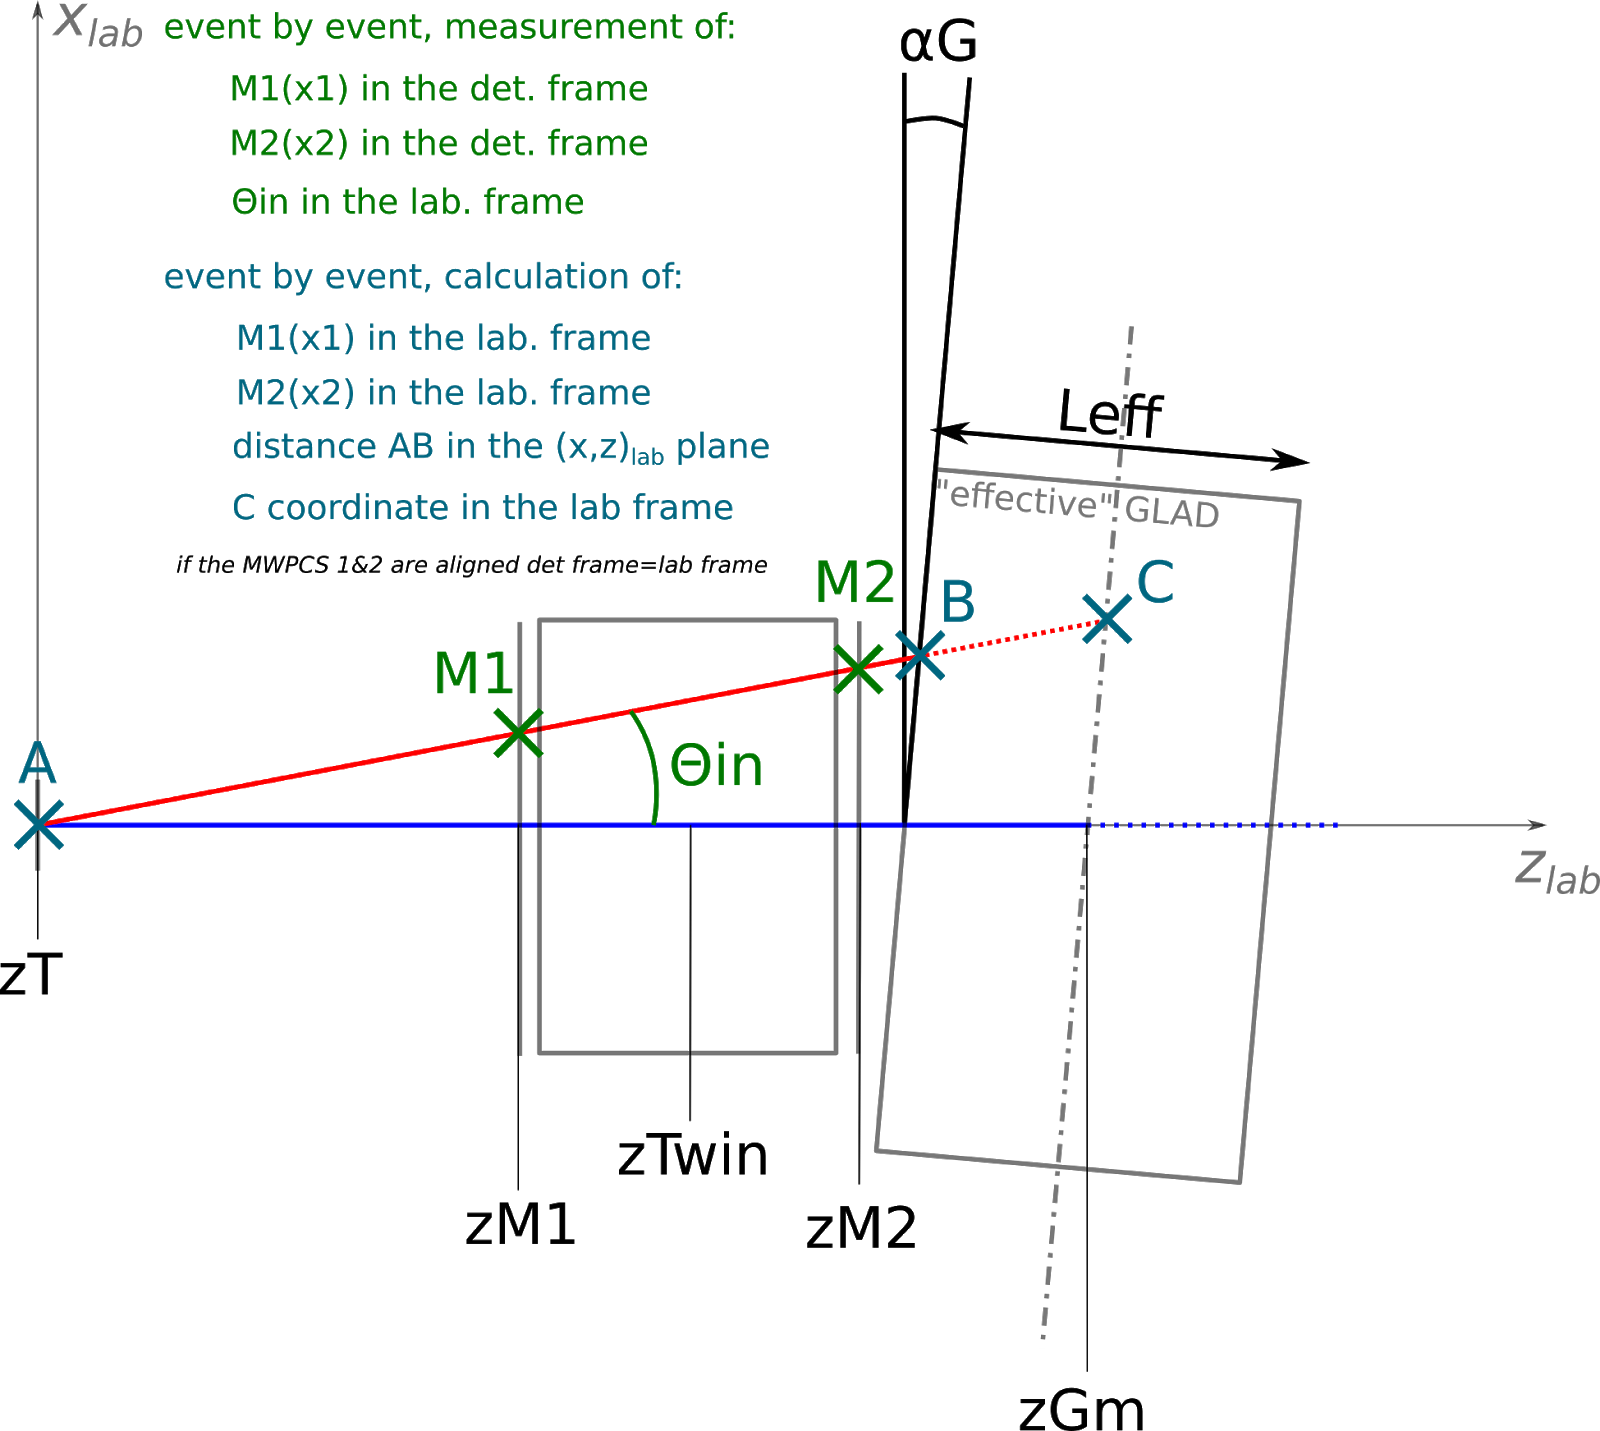
\includegraphics[width=1.2\textwidth]{tracking_upstreamGLAD.png}
\end{center}
\textbf{The straight line trajectory from MW0 to  entrance before glad is defined by:}\\
\textbf{$\Rightarrow$ one absolute value before GLAD}\\
absolute = calibrated position in mm in the laboratory frame\\
To get the position, use the position given by one MWPCs (1 or 2)\\
\\
\textbf{$\Rightarrow$ the theta angle (theta\textunderscore in) before GLAD}\\
Angle obtained from comining MWPC1 and MWPC2\\
(to get higher precision the drift time in TWIM MUSIC could be used)\\
\subsubsection{From entrance to the exit of GLAD, the effective trajectory is circular}
\begin{center}
	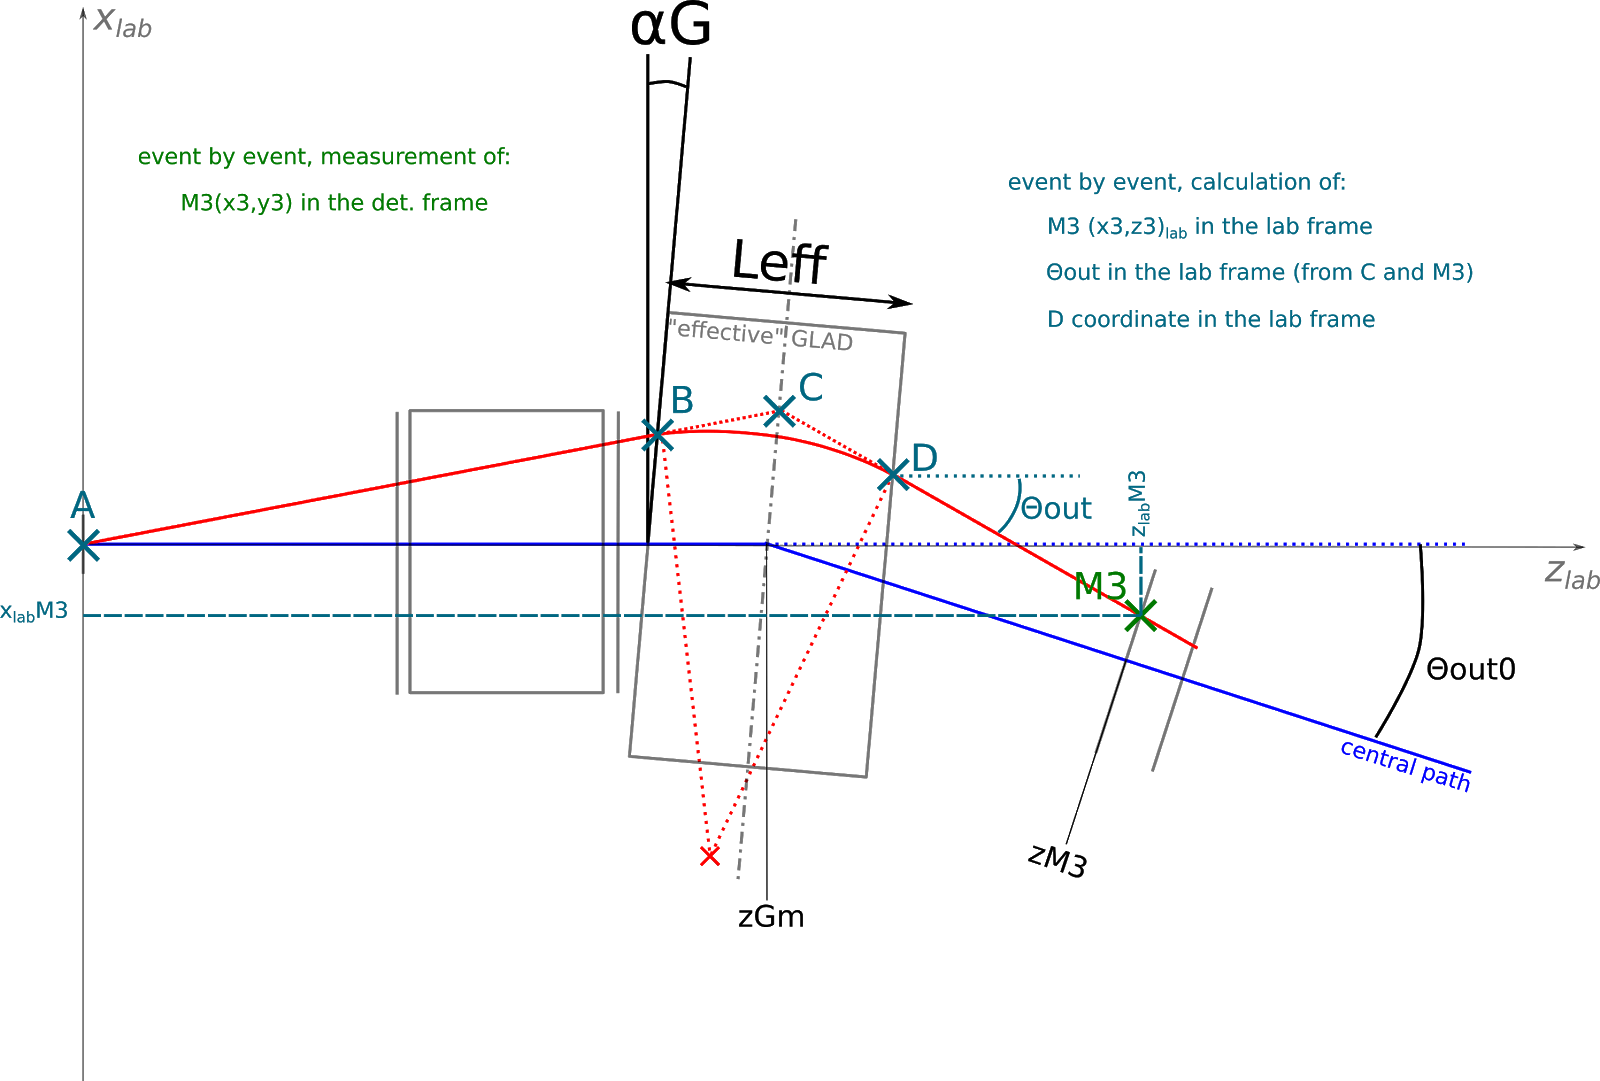
\includegraphics[width=1.2\textwidth]{tracking_GLAD.png}
\end{center}
\textbf{The circular trajectory is defined by:\\
$\Rightarrow$ one absolute position before GLAD B and angle theta\textunderscore in (see: \ref{sssec:num1})\\
$\Rightarrow$ one absolute position at MWPC3}\\
\\
From this information the angle theta\textunderscore out is constructed in follwing steps:\\
\begin{enumerate}
	\item Extend the straight flightline of the ion before the GLAD.
	\item The point of intersection with the "kickplane" (symmetry axis line of GLAD magnet) is the kickpoint C.
	\item Draw a straight line between C and the absolute position at MWPC3 = M3.
	 \item theta\textunderscore out is the positive angle between the z-beam direction and the line between C and M3.
\end{enumerate}
The curvature radius $\rho$ is given by:\\
$\rho$ = $\frac{\textrm{L\textunderscore eff}}{2\cdot\sin\left(\frac{theta\textunderscore in}{2} +\frac{theta\textunderscore out}{2}\right)\cdot\cos(\delta)}$\\
\\
With $\delta$: \\
$\delta = \arctan\left( \Bigg| \frac{\frac{cos(theta\textunderscore out)-\cos(theta\textunderscore in)}{\sin(theta\textunderscore out)+\sin(theta\textunderscore in)}+\tan(\alpha)}{1-\frac{cos(theta\textunderscore out)-\cos(theta\textunderscore in)}{\sin(theta\textunderscore out)+\sin(theta\textunderscore in)}\cdot\tan(\alpha)}\Bigg| \right)$ \\
The full derivation can be found in the appendix.\\
\\
The circular trajectory is given by:\\
$\omega = 2*\Bigg|\arcsin\Big[\frac{BD}{2\cdot\rho}\Big] \Bigg|$\\
\\
with BD = length of the BD segment\\
\subsubsection{After GLAD up to the TOFW, the trajectory is a straight line}
\begin{center}
	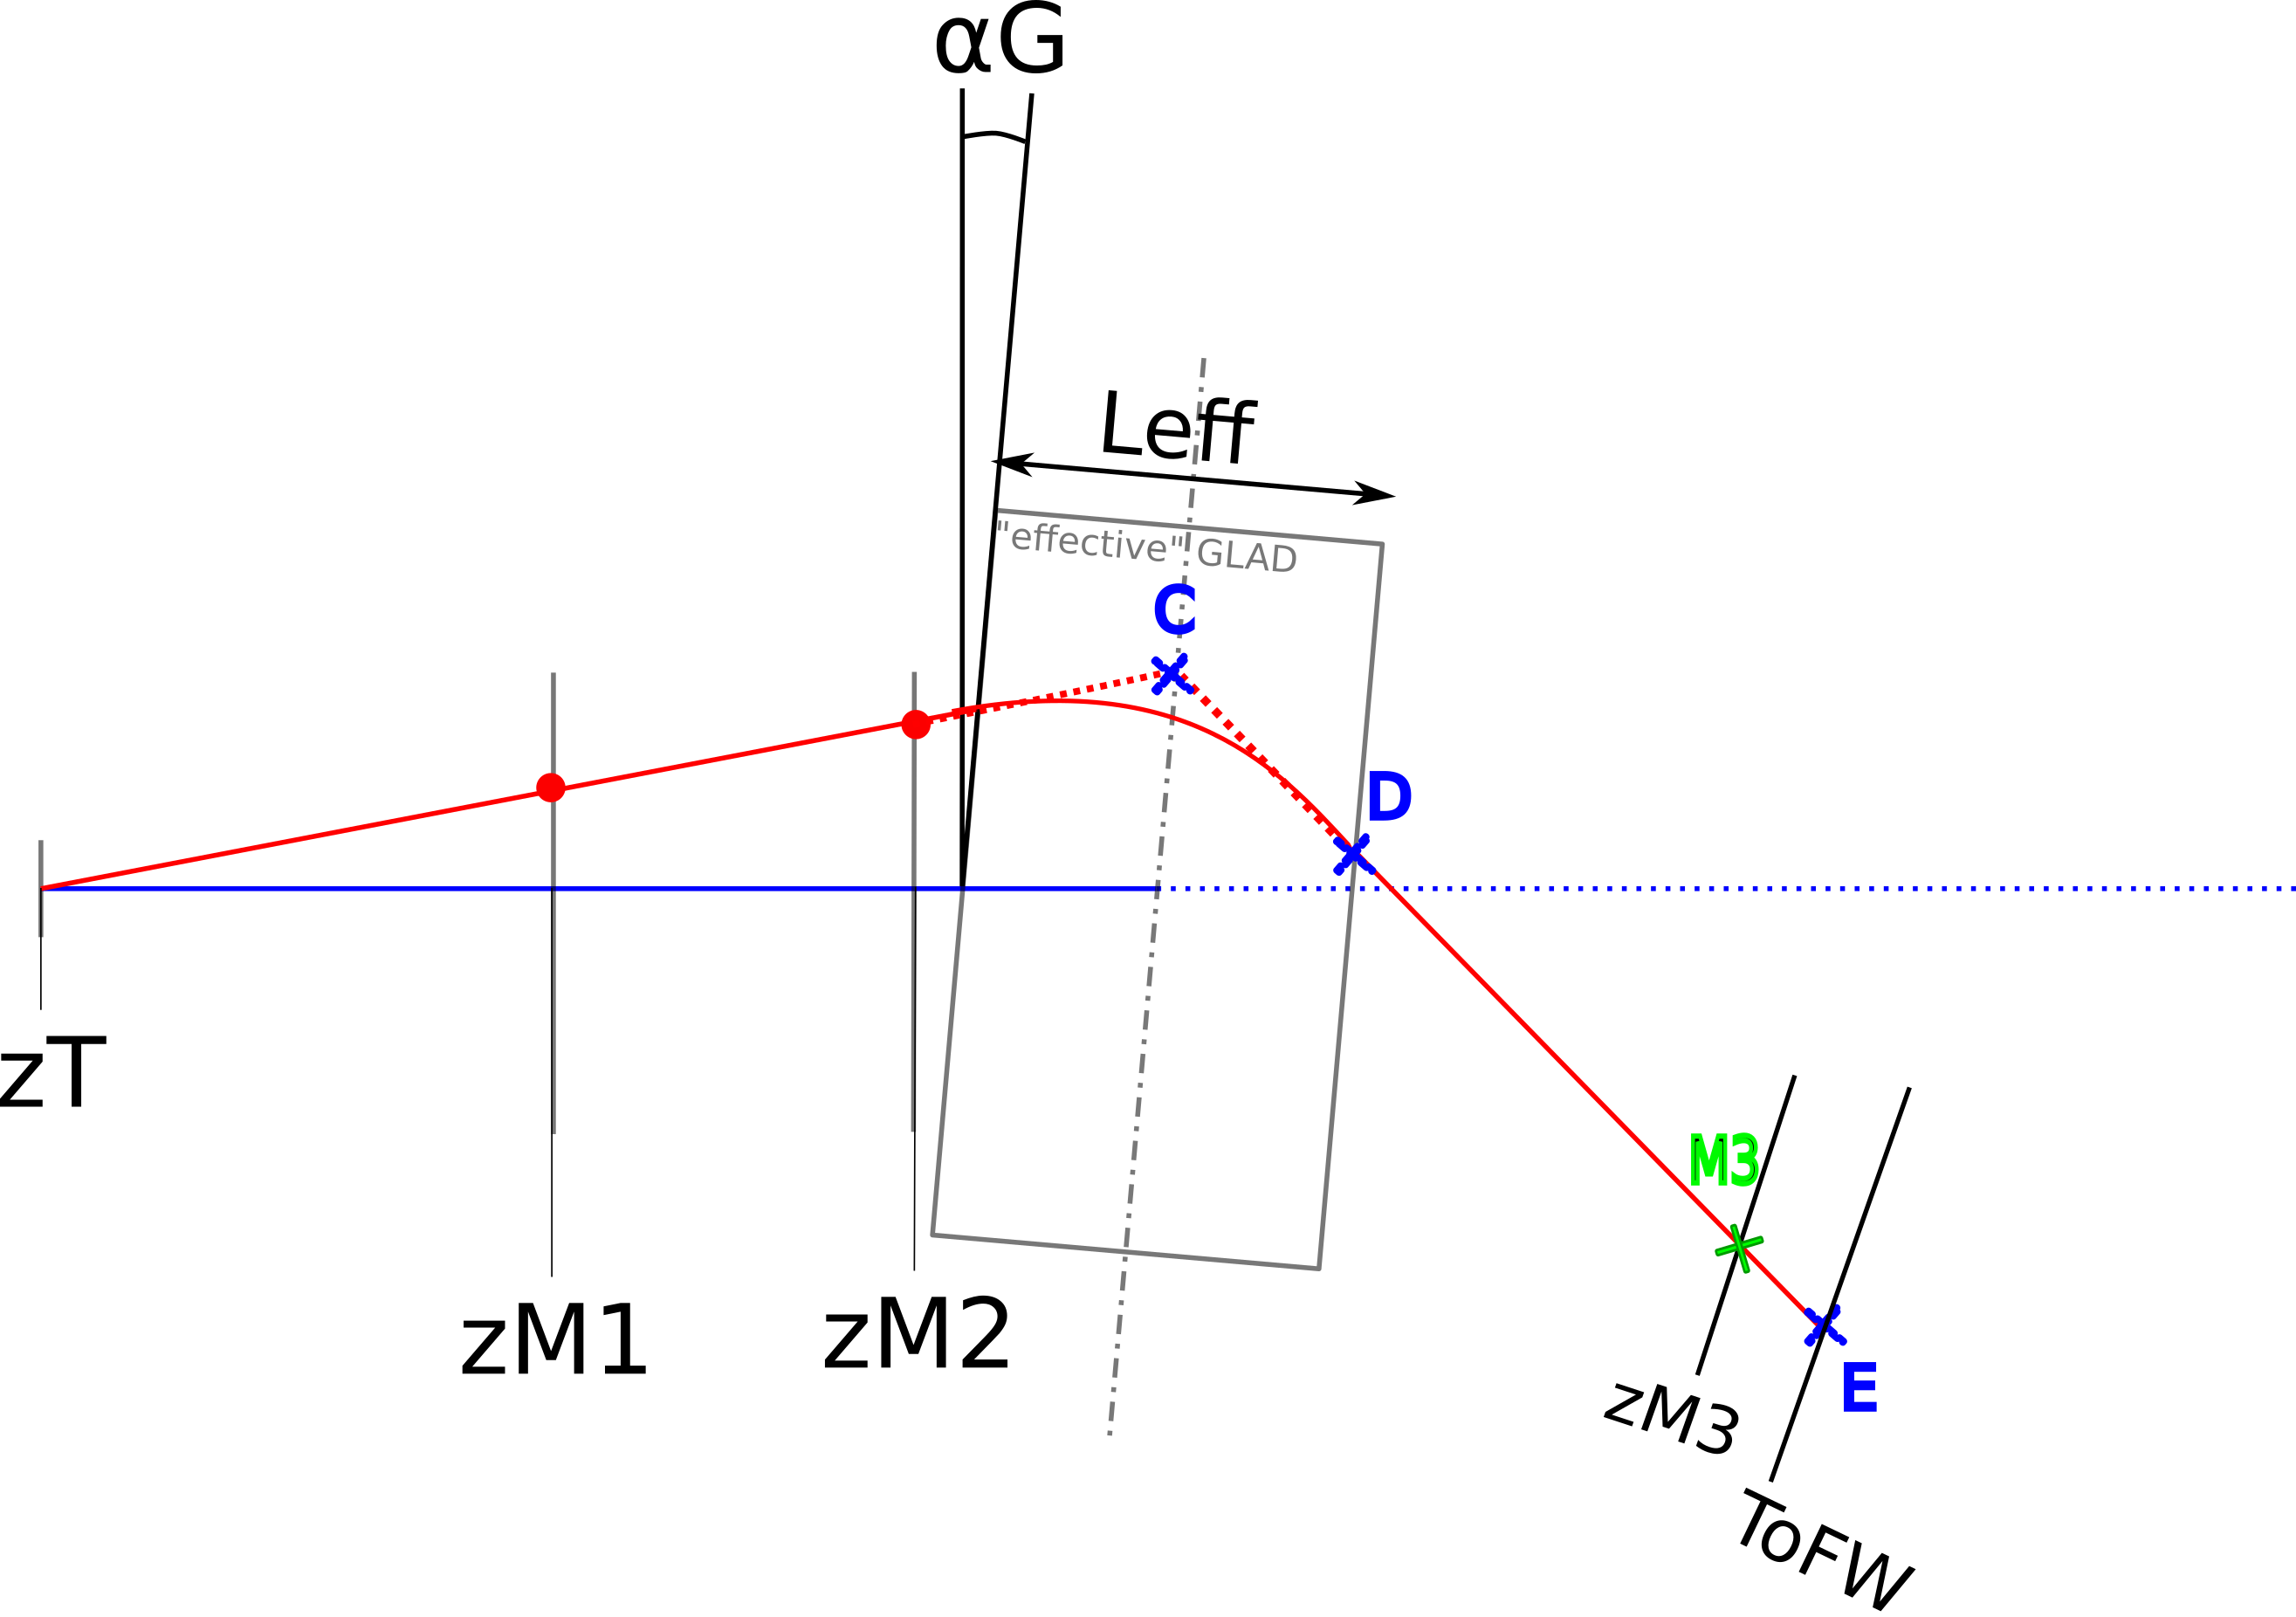
\includegraphics[width=1.2\textwidth]{tracking_downstreamGLAD.png}
\end{center}
\textbf{The straight line trajectory from D to E is definded by:}\\
\\
\textbf{$\Rightarrow$ the output angle from GLAD theta\textunderscore out}\\
\textbf{$\Rightarrow$ one absolute position after GLAD in the laboratory frame M3}\\
\\
With this information the straight line trajectory lenght after GLAD can be measured. It starts at the exit point of GLAD D and follows the straigh line (characterized by the angle theta\textunderscore out and the absolute position at MWPC3) until the intersection with the TofW ( middle position of the ToFWall zToFW$=6660.2 mm$, tilted angle$=18^{\circ}$).\\
\\
Finally the pathlength in the (x,z) plane from the target position to the ToFW is given by:\\
P = AB + $\rho\cdot\omega$ +DE\\
\\
where:\\
A = (x,z) position at the target point \\
B = (x,z) position at the GLAD entry point\\
D = (x,z) position at the GLAD exit point\\
E = (x,z) position where the constructed trajectory line hits the ToFW\\
\\
The assumption in the "Kickplane" method is that the kickpoint for each event lies on the predefinded Kickplane, the symmetry axis line of the GLAD magnet. 

\subsection{The "Fit-Track" method}
\subsection{The "Optic correction" method}






\end{document}